\documentclass[12pt]{article}
\usepackage[a4paper, total={5.5in, 9in}]{geometry}
\usepackage{amsmath}
\usepackage{changepage}
\usepackage[most]{tcolorbox}
\usepackage{textcomp}
\usepackage{tikz}
\usepackage{pgfplots}
\pgfplotsset{compat=1.18}
\usepackage{amsfonts}
\usepackage{graphicx}

\title{Precalculus Worksheet 8.3}
\author{PCL Learning Center}
\date{}

\begin{document}
\maketitle

\begin{center}
    \textit{note: No graphing calculators or electronic devices may be used on this worksheet.}    
\end{center}

\section*{Problem Set 1\\Difficulty level: Normal}
\subsection*{Problem 1}
What are the polar coordinates \((r,\theta)\) of the point \(B\) shown below?

\begin{figure}[!ht]
    \centering
    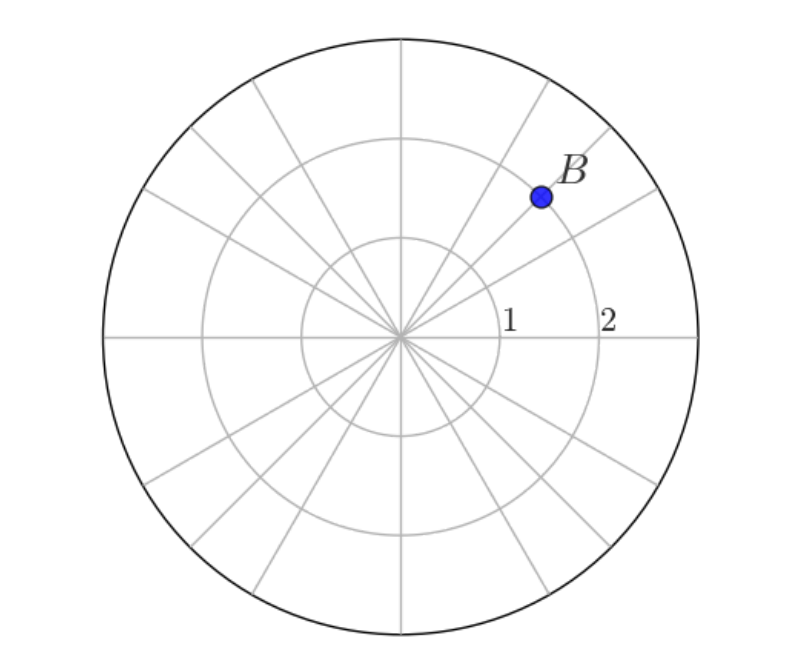
\includegraphics[width=0.5\linewidth]{polar_point_1.png}
\end{figure}

\subsection*{Problem 2}
Write the polar coordinates \((-8,\dfrac{7\pi}{6})\) as rectangular coordinates.

\subsection*{Problem 3}
Given the point \((10,\dfrac{\pi}{3})\) in polar coordinates, what are the Cartesian coordinates of the point?

\subsection*{Problem 4}
Given the point with Cartesian coordinates \((-4,-4\sqrt{3})\), find the polar coordinates of the point.

\subsection*{Problem 5}
Find the polar coordinates of a point with Cartesian coordinates \((x,y)=(9,0)\).

\subsection*{Problem 6}
Convert the given Cartesian equation into a polar equation.
\[y=3x+5\]

\subsection*{Problem 7}
Convert the given polar equation into a Cartesian equation.
\[r=7\sin \theta + 9\cos \theta\]

\subsection*{Problem 8}
Convert the given polar equation into a Cartesian equation.
\[r=6\sin \theta + 9\cos \theta\]

\subsection*{Problem 9}
Which of the following points has the same location as point \(A\) with polar coordinates \((-2,\dfrac{11\pi}{6})\)?

    \begin{itemize}
        \item[(a)] \(\left( -2, -\dfrac{\pi}{6} \right)\)
        \item[(b)] \(\left( 2, -\dfrac{11\pi}{6} \right)\)
        \item[(c)] \(\left( 2, \dfrac{5\pi}{6} \right)\)
        \item[(d)] \(\left( 2, \dfrac{7\pi}{6} \right)\)
        \item[(e)] \(\left( -2, \dfrac{7\pi}{6} \right)\)
    \end{itemize}

\section*{Problem Set 2\\Difficulty level: Hard}
\subsection*{Problem 1}
How are the polar axes different from the \(x-\) and \(y-\) axes of the Cartesian plane?

\subsection*{Problem 2}
Explain why the points \((-3,\dfrac{\pi}{2})\) and \((3,-\dfrac{\pi}{2})\) are the same.

\newpage
\section*{Solutions for the Set 1}
\subsection*{Problem 1}
\((2,\dfrac{\pi}{4})\)
\subsection*{Problem 2}
\((4\sqrt{3},4)\)
\subsection*{Problem 3}
\((5,5\sqrt{3})\)
\subsection*{Problem 4}
\((8,\dfrac{4\pi}{3})\)
\subsection*{Problem 5}
\((9,2\pi)\)
\subsection*{Problem 6}
\(r=\dfrac{5}{\sin \theta -3\cos \theta}\)
\subsection*{Problem 7}
\(x^2+y^2=9x+7y\)
\subsection*{Problem 8}
\(x^2+y^2=9x+6y\)
\subsection*{Problem 9}
    \begin{itemize}
        \item[(a)] \(\left( -2, -\dfrac{\pi}{6} \right)\)
        \item[(b)] \(\left( 2, -\dfrac{11\pi}{6} \right)\)
        \item[(c)] \(\left( 2, \dfrac{5\pi}{6} \right)\)
    \end{itemize}
    
\section*{Solutions for the Set 2}
\subsection*{Problem 1}
The polar system uses a distance and angle from a point, while the Cartesian system uses perpendicular distances from two axes.
\subsection*{Problem 2}
The points \((-3,\dfrac{\pi}{2})\) and \((3,-\dfrac{\pi}{2})\) are the same because they lie on the same line but in opposite directions, and the negative radius reverses the direction of the angle.
\end{document}
